%% This is an example first chapter.  You should put chapter/appendix that you
%% write into a separate file, and add a line \include{yourfilename} to
%% main.tex, where `yourfilename.tex' is the name of the chapter/appendix file.
%% You can process specific files by typing their names in at the 
%% \files=
%% prompt when you run the file main.tex through LaTeX.
\chapter{Evaluation}
All evaluation was done on a Mid 2012 15 inch MacBook Pro with 2.7 Ghz Intel Core i7 processor and 16GB of RAM. All VMs were running on the same host, though VM2Docker makes no such restriction in practice, as only the IP address of each VM is required. The practical convenience of running on the same host allowed for a drastic speed improvement when transferring the entire VM's filesystem over the socket from agent to chief, as opposed to over a potentially slow network connection.
\label{chap:eval}
% Different OS's, network latency, etc
\section{Conversion Time}
% note about solid state drives, network latency, etc
\section{Disk Usage}
\begin{table}[h]
\centering
    \begin{tabular}{| c | c | c | c | c | c | c |}
    \hline
& \multicolumn{5}{|c|}{\bfseries Ubuntu Server} \\ \hline
    \bfseries Release & \itshape 12.04 & \itshape 13.04 & \itshape 13.10 & \itshape 14.04 & \itshape 14.10 \\ \hline
    \bfseries VM & 1125.8 & 876.4 & 1157.5 & 1212.2 & 1132.2\\ \hline
    \bfseries Base Image & 99.1 & 160.4 & 114.8 & 192.0 & 196.9  \\ \hline
    \bfseries rsync & 996.7 & 710.9 & 982.4 & 1008.9 & 876.4\\ \hline 
    \bfseries rdiff & 974.4 & 718.2 & 987.3 & 971.2 & 872.5\\ \hline 
    \end{tabular}
\caption{}
\label{table:diff}
\end{table}

\begin{table}[h]
\centering
    \begin{tabular}{| c | c | c | c |}
    \hline
& \multicolumn{3}{|c|}{\bfseries CentOS Minimal} \\ \hline
    \bfseries Release & \itshape 5* & \itshape 6 & \itshape 7 \\ \hline
    \bfseries VM & 2543.8 &  676.0 & 881.7\\ \hline
    \bfseries Base Image & 496.0 & 236.1 & 243.1\\ \hline
    \bfseries rsync & 2190.0 & 478.1 & 704.1\\ \hline 
    \bfseries rdiff & 2138.7 & 416.7 & 621.7\\ \hline 
    \end{tabular}
\caption{}
\label{table:diff}
\end{table}

\begin{table}[h]
\centering
    \begin{tabular}{| c | c | c |}
    \hline
& \multicolumn{2}{|c|}{\bfseries Mageia Minimal} \\ \hline
    \bfseries Release & \itshape 3 & \itshape 4*  \\ \hline
    \bfseries VM & 738.4 & 2808.4 \\ \hline
    \bfseries Base Image & 160.4 & 174.1\\ \hline
    \bfseries rsync & 595.1 & 2575.4\\ \hline 
    \bfseries rdiff & 581.0 & 2613.0\\ \hline 
    \end{tabular}
\caption{}
\label{table:diff}
\end{table}



\subsection{rsync}

\subsection{rdiffdir}
%http://librsync.sourcefrog.net/doc/rdiff.html
\section{Package Management}

% data tables that include package installation
\begin{table}[h]
\centering
    \begin{tabular}{| c | c | c | c | c |}
    \hline
& \multicolumn{4}{|c|}{\bfseries Ubuntu Server} \\ \hline
    \bfseries Release & \itshape 12.04 & \itshape 13.10 & \itshape 14.04 & \itshape 14.10 \\ \hline
    \bfseries VM & 1125.8 & 1157.5 & 1212.2 & 1132.2\\ \hline
    \bfseries Base Image & 99.1 & 114.8 & 192.0 & 196.9  \\ \hline
    \bfseries BI + Packages & 326.4 & 447.7 & 386.9 & 468.6  \\ \hline
    \bfseries rsync & 902.2 & 767.7 & 894.8 & 687.6\\ \hline 
    \bfseries rdiff & 810.9 & 708.1 & 829.0 & 655.0\\ \hline \hline
     \bfseries \% rsync & 41.6 & 64.5 & 58.5 & 69.5\\ \hline
 \bfseries \% rdiff & 71.9 & 83.9 & 73.0 & 80.0\\
    \hline
    \end{tabular}
\caption{Note 13.04 is missing due to a repository error at the time of data colleciton. Important figures here to note are the \% redeuction in diff size relative to the increase in base image + package size. Anything that is not 100\% is a theoretical increase in total size of the Docker image, but with layering across multiple containers that share the same lineage, this ends up cancelling out.}
\label{table:diff}
\end{table}

\begin{table}[h]
\centering
    \begin{tabular}{| c | c | c | c |}
    \hline
& \multicolumn{2}{|c|}{\bfseries CentOS} & \multicolumn{1}{|c|}{\bfseries Mageia} \\ \hline
    \bfseries Release & \itshape 6 & \itshape 7 & \itshape 3 \\ \hline
    \bfseries VM & 676.0 & 881.7 & 738.4\\ \hline
    \bfseries Base Image & 236.1 & 243.1 & 160.4  \\ \hline
    \bfseries BI + Packages & 522.6 & 660.2 & 704.6 \\ \hline
    \bfseries rsync & 381.9 & 544.5 & 535.9 \\ \hline 
    \bfseries rdiff & 269.4 & 370.9 & 417.7 \\ \hline \hline
     \bfseries \% rsync & 33.6 & 38.3 & 10.9 \\ \hline
 \bfseries \% rdiff & 51.4 & 60.1 & 30.0 \\
    \hline
    \end{tabular}
\caption{}
\label{table:diff}
\end{table}



\begin{table}[h]
\centering
\label{table:culling}
    \begin{tabular}{| c | c | c | c | c | c | c | c | c |}
    \hline
& \multicolumn{5}{|c|}{\bfseries Ubuntu Server} & \multicolumn{2}{|c|}{\bfseries CentOS} & \multicolumn{1}{|c|}{\bfseries Mageia} \\ \hline
    \bfseries Release & \itshape 12.04 & \itshape 13.04 & \itshape 13.10 & \itshape 14.04 & \itshape 14.10  & \itshape 6 & \itshape 7 & \itshape 3 \\ \hline
    \bfseries Before & 205 & 226 & 248 & 183 & 245 & 78 & 165 & 311\\ \hline
    \bfseries After & 67 & 129 & 147 & 109 & 144 & 54 & 67 & 46   \\ \hline \hline
    \bfseries \% Saved & 67.3 & 42.9 & 40.7 & 40.4 & 41.2 & 30.8 & 59.4 & 85.2\\
    \hline
    \end{tabular}
\caption{Results of package culling}
\label{table:diff}
\end{table}
\section{Container Performance}
\newpage
\clearpage
\newpage
\section{Evaluation Strategy}
\subsection{System Diagram}

\begin{figure}[h]
\centering
    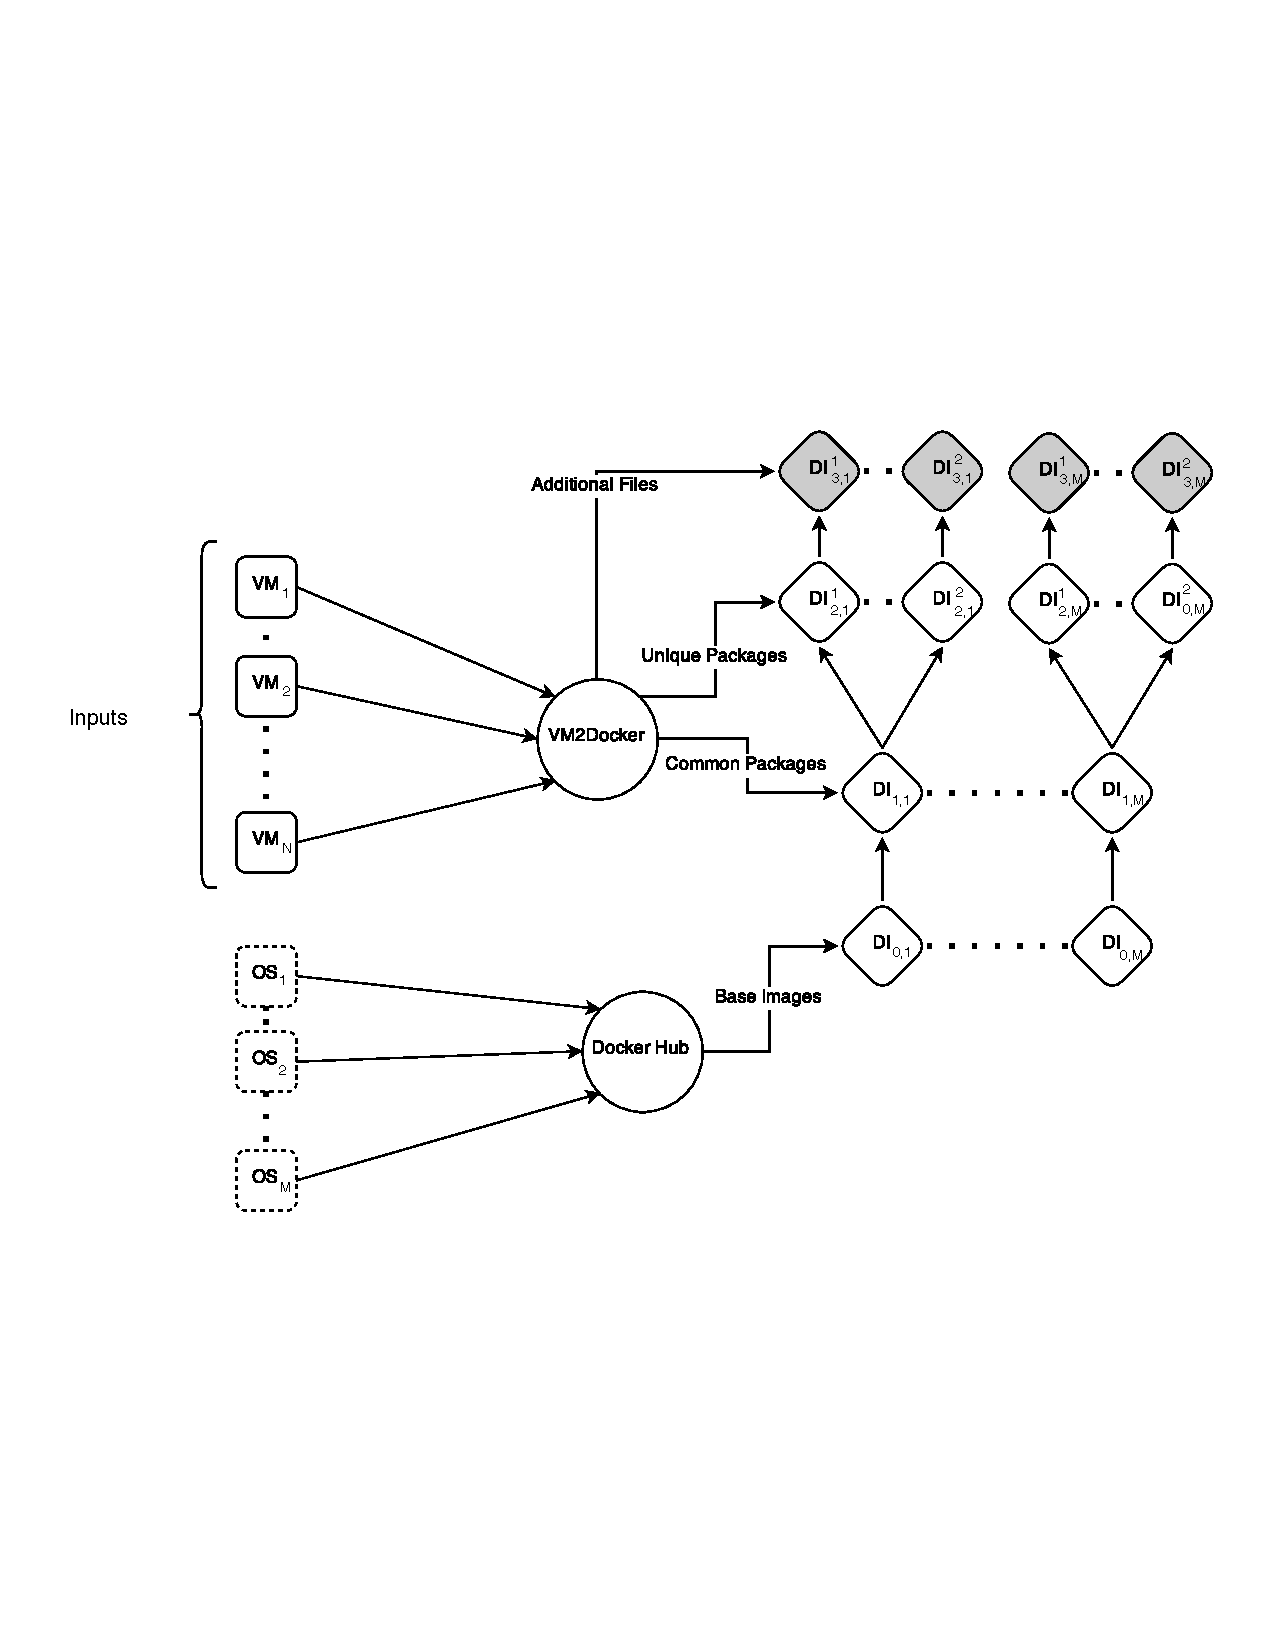
\includegraphics[width=1.0\textwidth]{system.pdf}
    \caption{The following diagram illustrates an overview of the system and how the VM2Docker framework interacts with the virtual machines provided as input and converts them to corresponding, layered, Docker containers. The rounded squares represent the input virtual machines, the circles correspond to immutable programs that interact with the inputs or outputs in some way, and the rounded diamonds represent the resulting Docker images. Each image consists of a series of layers, which is illustrated by starting at the given image and traversing the links backwards to the base image ($DC_0$). The final images, equal to the original VM filesystem, are represented by the shaded diamonds ($DC_3$). The number of these is exactly equal to N, the original number of VMs to be converted.}
\end{figure}
%$\text{DC}_3$)
% ($\text{DC}_0$)

\underline{VM}\\
The VMs are the inputs provided to the library. They are fully functioning virtual machines with as many or as few packages and additional files installed as needed. They must be running a Linux-based operating system with Kernel version $\ge$ 3.8. Any OS beyond that is theoretically supported; however, VM2Docker has been only tested to work with Ubuntu, CentOS, and Mageia. Support for additional OSs is achieved by subclassing the appropriate base class and overriding a small set of OS-specific commands and parameters.

\underline{OS}\\
Each OS is an operating system and specific release that corresponds to the set of VMs provided as input. Therefore $M \le N$. If all VMs provided as input are of the same operating system and release, then $M=1$. Ubuntu, CentOS, and Mageia were specifically chosen because the publicly accessible "Docker Hub" has base images available for many of the major releases of these operating systems.


\underline{Base Images}\\
Base images are watered-down versions of a given release of an Operating System and range in size between 100 and 200 MB. They do not contain the kernel. They are represented by $DC_0$ in the diagram

\underline{Common package images}\\
The next layer, $DC_1$, consists of a given base image with the set of packages installed that are common to all VMs of a given operating system release in the set of VMs provided as input.

\underline{Unique packages}\\
The next layer, $DC_2$, consists of the installation of additional packages, on top of the common packages, that are not in the intersection of software for a given operating system release.

\underline{Additional Files}\\
The final step in the conversion of files is performing a filesystem diff from the previous layer, $DC_2$ to the original VM. The final layer $DC_3$ contains this diff and is therefore identical to the original VM in terms of its files.

\subsection{Expected Use Cases}
It is very hard to describe what might be an "average" looking input to this system because one could use a Virtual Machine to do a wide range of computing. Nonetheless, there are many real-world practical use cases where VM2Docker might be particularly effective. The class of VMs that are used as servers in a simple client-server interaction are one example of such inputs. A given VM might be running a webserver, database, mail server, or other server-based daemon and might represent one such input to the VM2Docker system. 

\subsection{Experiments}
For the following set of experiments, we will assume that $M=1$ in the following diagram. This will greatly reduce the number of experiments to be run as well as simplify the understanding of the system diagram in each case. Each distinct operating system does not share any resulting image layers in common because the first layer, the base image ($DC_0$), is OS and release-specific. Thus, restricted our set of inputs such that all VMs share the same OS and release ($M=1$) does not drastically alter the results and instead represents a narrowing of scope to a single tree of image layers, pictured on the right in the diagram. The results for $M>1$ can be therefore obtained by merging the results from a set of $M$ independent experiments each of which $M=1$.

All of the following single VM experiments have already been executed. Their results are included above. With only one VM provided as input, $DC_1$ and $DC_2$ are indistinguishable. We will assume $DC_2$ has a delta size of 0 MB, and include the statistics for $DC_1$ and $DC_3$. These inputs can be considered the base cases.

\begin{enumerate}


\item 1 VM, Ubuntu 12.04 Server Edition\\
VM Size: 1125.8 MB\\
VM Size - kernel: 1023.6 MB\\

VM is the simple server edition downloaded from the Ubuntu website with nothing else additional installed or added.\\

$DC_0$ is 99.1 MB\\
Results:\\
$DC_1$: 227.3 MB\\
$DC_3$: 708.7 MB\\

\item 1 VM, Ubuntu 13.10 Server Edition\\
VM Size: 1157.5 MB\\
VM Size - kernel: 1055.2 MB\\

VM is the simple server edition downloaded from the Ubuntu website with nothing else additional installed or added.\\

$DC_0$ is 114.8 MB\\
Results:\\
$DC_1$: 332.9 MB\\
$DC_3$: 605.8 MB\\

\item 1 VM, Ubuntu 14.04 Server Edition\\
VM Size: 1212.2 MB\\
VM Size - kernel: 1109.9 MB\\

VM is the simple server edition downloaded from the Ubuntu website with nothing else additional installed or added.\\

$DC_0$ is 192.0 MB\\
Results:\\
$DC_1$: 194.9 MB\\
$DC_3$: 726.7 MB\\

\item 1 VM, Ubuntu 14.10 Server Edition\\
VM Size: 1132.2 MB\\
VM Size - kernel: 1029.9 MB\\

VM is the simple server edition downloaded from the Ubuntu website with nothing else additional installed or added.\\

$DC_0$ is 196.9 MB\\
Results:\\
$DC_1$: 271.7 MB\\
$DC_3$: 552.7 MB\\
\item 1 VM, CentOS 6 Minimal Edition\\
VM Size: 676.0 MB\\
VM Size - kernel: 573.7 MB\\

VM is the simple server edition downloaded from the Ubuntu website with nothing else additional installed or added.\\

$DC_0$ is 236.1 MB\\
Results:\\
$DC_1$: 286.5 MB\\
$DC_3$: 157.1 MB\\
\item 1 VM, CentOS 7 Minimal Edition\\
VM Size: 881.7 MB\\
VM Size - kernel: 779.4 MB\\

VM is the simple server edition downloaded from the Ubuntu website with nothing else additional installed or added.\\

$DC_0$ is 243.1 MB\\
Results:\\
$DC_1$: 417.1 MB\\
$DC_3$: 268.6 MB\\
\item 1 VM, Mageia 3\\
VM Size: 738.4 MB\\
VM Size - kernel: 636.1 MB\\

VM is the simple server edition downloaded from the Ubuntu website with nothing else additional installed or added.\\

$DC_0$ is 160.4 MB\\
Results:\\
$DC_1$: 544.2 MB\\
$DC_3$: 315.4 MB\\

Each of the base case experiments represent a relatively "clean" VM with a minimal amount of packages installed. An optimal conversion would be one such that the size of $DC_3$ is as close to 0 as possible. This would imply that the package extraction and reinstallation process is efficient and 100\% effective. In practice, the size of $DC_3$ is non-zero, although greatly reduced from the original size of the VM. There are a few practical limitations of the package detection and reinstallation process that can account for these results. Due to the automatic detection of packages and reinstallation on top of $DC_0$ with auto-generated commands, it is likely that some, but not all, of the packages that are reinstalled are not identical byte-for-byte versions of the original packages that were installed on the VM. This can be due to a difference in version number, release, or some other subtle difference in the installation process. This would result in some or all of a given package to still exist in the "additional files" component of $DC_3$. There is also a host of software and files that can't necessarily be reinstalled from the default package management tool for the given OS. Cache files, too, can sometimes account for 50-100 MB of files in the original VM.

\item 2VMs

$VM_1$: CentOS6 Minimal, 676 MB\\
$VM_2$: CentOS6 Complete Install, 2.8 GB\\

The difference between these two VMs is additional packages and repositories that are provided in the complete install. The second VM contains all of the packages on the first VM.

Expected outputs:\\

$DC_1$: 286.5 MB\\
$DC_2^1$: 0 MB\\
$DC_2^2$: $\sim$ 1.5 - 2 GB\\
$DC_3^1$: 157.1MB\\
$DC_3^2$: 300-500MB\\

The packages common to both VMs will be all those in the original $DC_1$ for the minimal CentOS 6 experiment. $DC_2$ and $DC_3$ for the first VM will be 0, and 157.1MB, respectively, because there will be no additional packages unique to the first VM that aren't on the second, and then the final additional files layer will remained unchanged. For $VM_2$, we should expect $DC_2$ to drastically increase in size to take into account all of the packages unique to the second VM. In practice, this should be responsible for the majority of the increase in space of the original VM. All other files will be located in $DC_3$. Since the reinstallation process isn't always perfect, we will expect to see an increase in size of this layer approximately proportional to the increase in size of $DC_2$.

\item 2VMs

$VM_1$: CentOS6 Minimal, 676 MB\\
$VM_2$: CentOS6 Minimal plus 300 MB of additional files scattered across the OS, 1000 MB\\

Expected outputs:\\

$DC_1$: 286.5 MB\\
$DC_2^1$: 0 MB\\
$DC_2^2$: 0 MB\\
$DC_3^1$: 157.1MB\\
$DC_3^2$: 457MB\\

The only differences between these two VMs comes in the addition of 300MB of files that can't be categorized into packages. This will result in an increase in $DC_3$ of the size of the additional files that were added to the VM.

\item 3VMs

$VM_1$: CentOS6 Minimal, 676 MB\\
$VM_2$: CentOS6 Minimal plus 300 MB of additional files scattered across the OS, 1000 MB\\
$VM_3$: CentOS6 Complete, 2.8 GB\\

Expected outputs:\\

$DC_1$: 286.5 MB\\
$DC_2^1$: 0 MB\\
$DC_2^2$: 0 MB\\
$DC_2^3$: $\sim$ 1.5 - 2 GB\\
$DC_3^1$: 157.1MB\\
$DC_3^2$: 457MB\\
$DC_3^3$: 300-500MB\\

These results should be a combination of the two previous 2VM experiments, with the sizes remaining the same as if the experiments were run separately.
\item 3VMs

$VM_1$: CentOS6 Minimal, 676 MB\\
$VM_2$: CentOS6 Complete plus 300 MB of additional files scattered across the OS, 3.1GB\\
$VM_3$: CentOS6 Complete, 2.8 GB\\

Expected outputs:\\

$DC_1$: 286.5 MB\\
$DC_2^1$: 0 MB\\
$DC_2^2$: $\sim$ 1.5 - 2 GB\\
$DC_2^3$: $\sim$ 1.5 - 2 GB\\
$DC_3^1$: 157.1MB\\
$DC_3^2$: 600-800MB\\
$DC_3^3$: 300-500MB\\

These results should be similar in practice to the previous experiment as well. An interesting feature of VM2Docker will be exposed here as well. Since $DC_2^2$ and $DC_2^3$ are the same, they will be only represented once on disk by the same image. This is thanks to an implicit feature of Docker. Since VM2Docker generates Dockerfiles, which are instructions to generate the image, the Dockerfiles for $DC_2^2$ and $DC_2^3$ will be the same (the commands are the same and they are installing the same packages). VM2Docker sorts the list of packages being installed to ensure that the command in the Dockerfile is the same on subsequent runs. 
\item 3VMs

$VM_1$: CentOS6 Minimal, 676 MB\\
$VM_2$: CentOS6 Complete, 2.8 GB\\
$VM_3$: CentOS6 Complete plus 1 more package of negligible size, 2.8 GB\\

Expected outputs:\\

$DC_1$: 286.5 MB\\
$DC_2^1$: 0 MB\\
$DC_2^2$: $\sim$ 1.5 - 2 GB\\
$DC_2^3$: $\sim$ 1.5 - 2 GB\\
$DC_3^1$: 157.1MB\\
$DC_3^2$: 600-800MB\\
$DC_3^3$: 300-500MB\\

These results will be the same as in the previous experiment, except that $DC_2^2$ and $DC_2^3$ will no longer occupy the same space on disk and will be two distinct images. This reveals a shortcoming of VM2Docker in its inability to execute multiple rounds of finding packages in common between multiple VMs. This will be addressed further in the discussion.
\end{enumerate}

\subsubsection{Explanation of Results}


\subsection{Discussion}




